% !TeX encoding = UTF-8
% !TeX spellcheck = pl_PL

% $Id:$

%Author: Wojciech Domski
%Szablon do ząłożeń projektowych, raportu i dokumentacji z sterowników robotów
%Wersja v.1.0.0
%


%% Konfiguracja:
\newcommand{\kurs}{Sterowniki robot\'{o}w}
\newcommand{\formakursu}{Projekt}

%odkomentuj właściwy typ projektu
\newcommand{\doctype}{Etap III}
%\newcommand{\doctype}{Raport}
%\newcommand{\doctype}{Dokumentacja}

%wpisz nazwę projektu
\newcommand{\projectname}{Miecz \'{S}wietlny}

%wpisz akronim projektu
\newcommand{\acronim}{Mi\'{S}}

%zmaiast X wpisz numer grupy projektowej
\newcommand{\nrgrupy}{4}
%wpisz Imię i nazwisko oraz numer albumu
\newcommand{\osobaA}{Patryk \textsc{Knapik}, 226302}
%w przypadku projektu jednoosobowego usuń zawartość nowej komendy
\newcommand{\osobaB}{Wojciech \textsc{Kosicki}, 234506}

%wpisz termin w formie, jak poniżej dzień, parzystość, godzina
\newcommand{\termin}{wtTP11}

%wpisz imię i nazwisko prowadzącego
\newcommand{\prowadzacy}{mgr in\.{z}. Wojciech \textsc{Domski}}

\documentclass[10pt, a4paper]{article}
% W nawiasie klamrowym podana jest klasa dokumentu. Standardowe klasy artykułu
% to: article, amsart, scrartcl, artikel1, artikel2, artikel3.
% W nawiasie prostokątnym deklarowane są opcje dokumentu. Zamiast 10pt
% można podać 11pt lub 12pt. Dokument w dwóch kolumnach uzyskuje się po
% wpisaniu opcji twocolumn, 

%Preambuła dokumentu

% linki w spisie tresci, bibliografi
\usepackage[bookmarks=true,bookmarksnumbered=false,unicode=true,pdftex=true, colorlinks,filecolor=black,linkcolor=black,urlcolor=black,citecolor=black]{hyperref}

%ustawienie rozmiaru papieru
\usepackage[a4paper, left=2.5cm, right=2.5cm, top=2.5cm, bottom=2.5cm, headsep=1.2cm]{geometry}

%rozmaite ustawienia pozwalające okreslić język

%NALEŻY wybrać jeden z pakietów
%\usepackage{polski} %przydatne podczas składania dokumentów w j. polskim
\usepackage[polish]{babel}  % pakiet lokalizujący dokument w języku polskim
%\usepackage[british]{babel}

\usepackage{indentfirst}	% polski styl pisania (np. rozpoczecie pierwszego akapitu
% pod nazwa rozdzialu od wciecia)
%\usepackage[OT4]{fontenc}
\usepackage[utf8]{inputenc} % w miejsce utf8 można wpisać latin2 bądź cp1250,
% w zależności od tego w jaki sposób kodowane są 
% polskie znaki diakrytyczne przy wprowadzaniu 
% z klawiatury.
%kodowanie znaków, zależne od systemu
\usepackage[T1]{fontenc} %poprawne składanie polskich czcionek

%OPEROWANIE NA OBRAZACH
\usepackage{graphicx}       % pakiet graficzny, umożliwiający m.in.
% import grafik w formacie eps
%\usepackage{epstopdf}		% pozwala na importowanie grafik w formacie eps
% przy użyciu pdflatex
\usepackage[update,prepend]{epstopdf}
\usepackage{rotating}       % pakiet umożliwiający obracanie rysunków
\usepackage{subfigure}      % pakiet umożliwiający tworzenie podrysunków
\usepackage{epic}           % pakiet umożliwiający rysowanie w środowisku latex
\usepackage{psfrag}         % pakiet umożliwiający podmianę łańcuchów znaków 
% w plikach eps
%\usepackage{curves}         % pakiet do wykreslania krzywych

%pakiety dodające dużo dodatkowych poleceń matematycznych
\usepackage{amsfonts}       % pakiet z rozmaitymi czcionkami matematycznymi
%\usepackage{amssymb}        % pakiet z rozmaitymi symbolami matematycznymi
\usepackage{amsmath}        % pakiet z rozmaitymi środowiskami matematycznymi

\usepackage{fp}             % pakiet z funkcjami operujacymi 
% na liczbach zmiennoprzecinkowych
\usepackage{calc}           % pakiet umożliwiający operacje arytmetyczne
% na tzw. licznikach (liczbach całkowitych)
\usepackage{leftidx}		% indeksy górne i dolne po lewej stronie

%definicje matematyczne
\providecommand{\abs}[1]{\lvert#1\rvert}
\providecommand{\norm}[1]{\lVert#1\rVert}

%pakiety wspomagające i poprawiające składanie tabel
\usepackage{supertabular}
\usepackage{array}
\usepackage{tabularx}
\usepackage{hhline}
\usepackage{longtable}		% wsparcie dla dlugich tabel
\usepackage{multicol}		% podzial strony na wiele kolumn

%pakiet do BibTex
\usepackage{cite}

\usepackage{url} %pakiet pozawalający na dodawanie adresów url w bibliografi

%pakiet wypisujący na marginesie etykiety równań i rysunków zdefiniowanych przez \label{}, chcąc wygenerować finalną wersję dokumentu wystarczy usunąć poniższą linię
%\usepackage{showlabels}

\usepackage{float}			% lepsza obsluga mechanizmow obiektow plywajacych
% wymuszenie wstawienia np. tabeli, obrazka w danym miejscu przez [H]

\usepackage{listings}       % pakiet dedykowany zrodlom programow
\usepackage{color}


\definecolor{dkgreen}{rgb}{0,0.6,0}
\definecolor{gray}{rgb}{0.5,0.5,0.5}
\definecolor{mauve}{rgb}{0.58,0,0.82}

\lstset{ %
	language=Matlab,                % the language of the code
	basicstyle=\scriptsize,           % the size of the fonts that are used for the code
	numbers=left,                   % where to put the line-numbers
	numberstyle=\tiny\color{gray},  % the style that is used for the line-numbers
	stepnumber=1,                   % the step between two line-numbers. If it's 1, each line 
	% will be numbered
	numbersep=5pt,                  % how far the line-numbers are from the code
	backgroundcolor=\color{white},      % choose the background color. You must add \usepackage{color}
	showspaces=false,               % show spaces adding particular underscores
	showstringspaces=false,         % underline spaces within strings
	showtabs=false,                 % show tabs within strings adding particular underscores
	%frame=single,                   % adds a frame around the code
	rulecolor=\color{black},        % if not set, the frame-color may be changed on line-breaks within not-black text (e.g. comments (green here))
	tabsize=2,                      % sets default tabsize to 2 spaces
	captionpos=b,                   % sets the caption-position to bottom
	breaklines=true,                % sets automatic line breaking
	breakatwhitespace=false,        % sets if automatic breaks should only happen at whitespace
	%title=\lstname,                   % show the filename of files included with \lstinputlisting;
	% also try caption instead of title
	keywordstyle=\color{blue},          % keyword style
	commentstyle=\color{dkgreen},       % comment style
	stringstyle=\color{mauve},         % string literal style
	escapeinside={\%*}{*)},            % if you want to add LaTeX within your code
	morekeywords={*,...},              % if you want to add more keywords to the set
	deletekeywords={...}              % if you want to delete keywords from the given language
}

%polish signs in lst code
\lstset{literate=%
	{ą}{{\k{a}}}1
	{ć}{{\'c}}1
	{ę}{{\k{e}}}1
	{ł}{{\l}}1
	{ń}{{\'n}}1
	{ó}{{\'o}}1
	{ś}{{\'s}}1
	{ż}{{\.z}}1
	{ź}{{\'z}}1
	{Ą}{{\k{A}}}1
	{Ć}{{\'C}}1
	{Ę}{{\k{E}}}1
	{Ł}{{\L}}1
	{Ń}{{\'N}}1
	{Ó}{{\'O}}1
	{Ś}{{\'S}}1
	{Ż}{{\.Z}}1
	{Ź}{{\'Z}}1
}

\usepackage{verbatim}       % pakiet dedykowany rozmaitym wydrukom tekstowym
\usepackage{ifthen}         % pakiet umożliwiający tworzenie prostych programów
% (m.in. zawiera instrukcje powtórzeniowe 
% i warunkowe)
\usepackage{upquote}		%normal quotations marks ' and `

% deklaracje wymagane przez pakiet theorem automatycznie ladowany w przypadku
% klasy dokumentu article
%
\newtheorem{Dn}{Definicja}[section]     % deklaracja srodowiska definicja
\newtheorem{La}[Dn]{Lemat}                % deklaracja srodowiska lemat
\newtheorem{Tm}[Dn]{Twierdzenie}          % deklaracja srodowiska twierdzenie
\newtheorem{Rk}[Dn]{Spostrze{\.z}enie}  % deklaracja srodowiska spostrzezenie
\newtheorem{Am}[Dn]{Algorytm}           % deklaracja srodowiska algorytm
\newtheorem{As}[Dn]{Za{\l}o{\.z}enie}   % deklaracja srodowiska zalozenie
\newtheorem{Pn}[Dn]{Propozycja}           % deklaracja srodowiska propozycja
\newtheorem{Py}[Dn]{W{\l}asno{\'s}{\'c}}  % deklaracja srodowiska wlasnosc
\newtheorem{Cy}[Dn]{Wniosek}              % deklaracja srodowiska wniosek
\newtheorem{Ee}[Dn]{Przyk{\l}ad}        % deklaracja srodowiska przyklad
\newtheorem{Ex}{{\'C}wiczenie}          % deklaracja srodowiska cwiczenie

%helps to specify width of a column in table
%\begin{tabular}{|C{1cm}|c|c|c|c|c|c|c|c|c|c|}
%first column will have widht of 1cm
\newcolumntype{L}[1]{>{\raggedright\let\newline\\\arraybackslash\hspace{0pt}}m{#1}}
\newcolumntype{C}[1]{>{\centering\let\newline\\\arraybackslash\hspace{0pt}}m{#1}}
\newcolumntype{R}[1]{>{\raggedleft\let\newline\\\arraybackslash\hspace{0pt}}m{#1}}

\sloppy			%zawija bardzo długie linie

%\pagenumbering{gobble}% Remove page numbers (and reset to 1)

	
\begin{document}

\def\tablename{Tabela}	%zmienienie nazwy tabel z Tablica na Tabela

\begin{titlepage}
	\begin{center}
		\textsc{\LARGE \formakursu}\\[1cm]		
		\textsc{\Large \kurs}\\[0.5cm]		
		\rule{\textwidth}{0.08cm}\\[0.4cm]
		{\huge \bfseries \doctype}\\[1cm]
		{\huge \bfseries \projectname}\\[0.5cm]
		{\huge \bfseries \acronim}\\[0.4cm]
		\rule{\textwidth}{0.08cm}\\[1cm]
		
		\begin{flushright} \large
		\emph{Skład grupy (\nrgrupy):}\\
		\osobaA\\
		\osobaB\\[0.4cm]
		
		\emph{Termin: }\termin\\[0.4cm]

		\emph{Prowadzący:} \\
		\prowadzacy \\
		
		\end{flushright}
		
		\vfill
		
		{\large \today}
	\end{center}	
\end{titlepage}

\newpage
\tableofcontents
\newpage

\section{Wstęp}
\label{sec:Wstęp}
Celem projektu jest skonstruowanie miecza świetlnego, który będzie wydawał charakterystyczne dźwięki zmieniające się w zależności od prędkości poruszania nim (efekt Doppler'a) raport opisuje jakie aspekty projektu udało się z powodzeniem zrealizować. Opisuje także ogólny przebieg prac oraz podjęte decyzje przy rozwiązywaniu problemów.

\section{Konfiguracja mikrokontrolera}
Pierwszym zadaniem było dobranie odpowiednich peryferiów wykorzystywanych w projekcie i skonfigurowanie ich w środowisku CubeMX. Wygenerowany kod był podstawą do rozpoczęcia pracy nad projektem.
\begin{figure}[H]
	\centering
	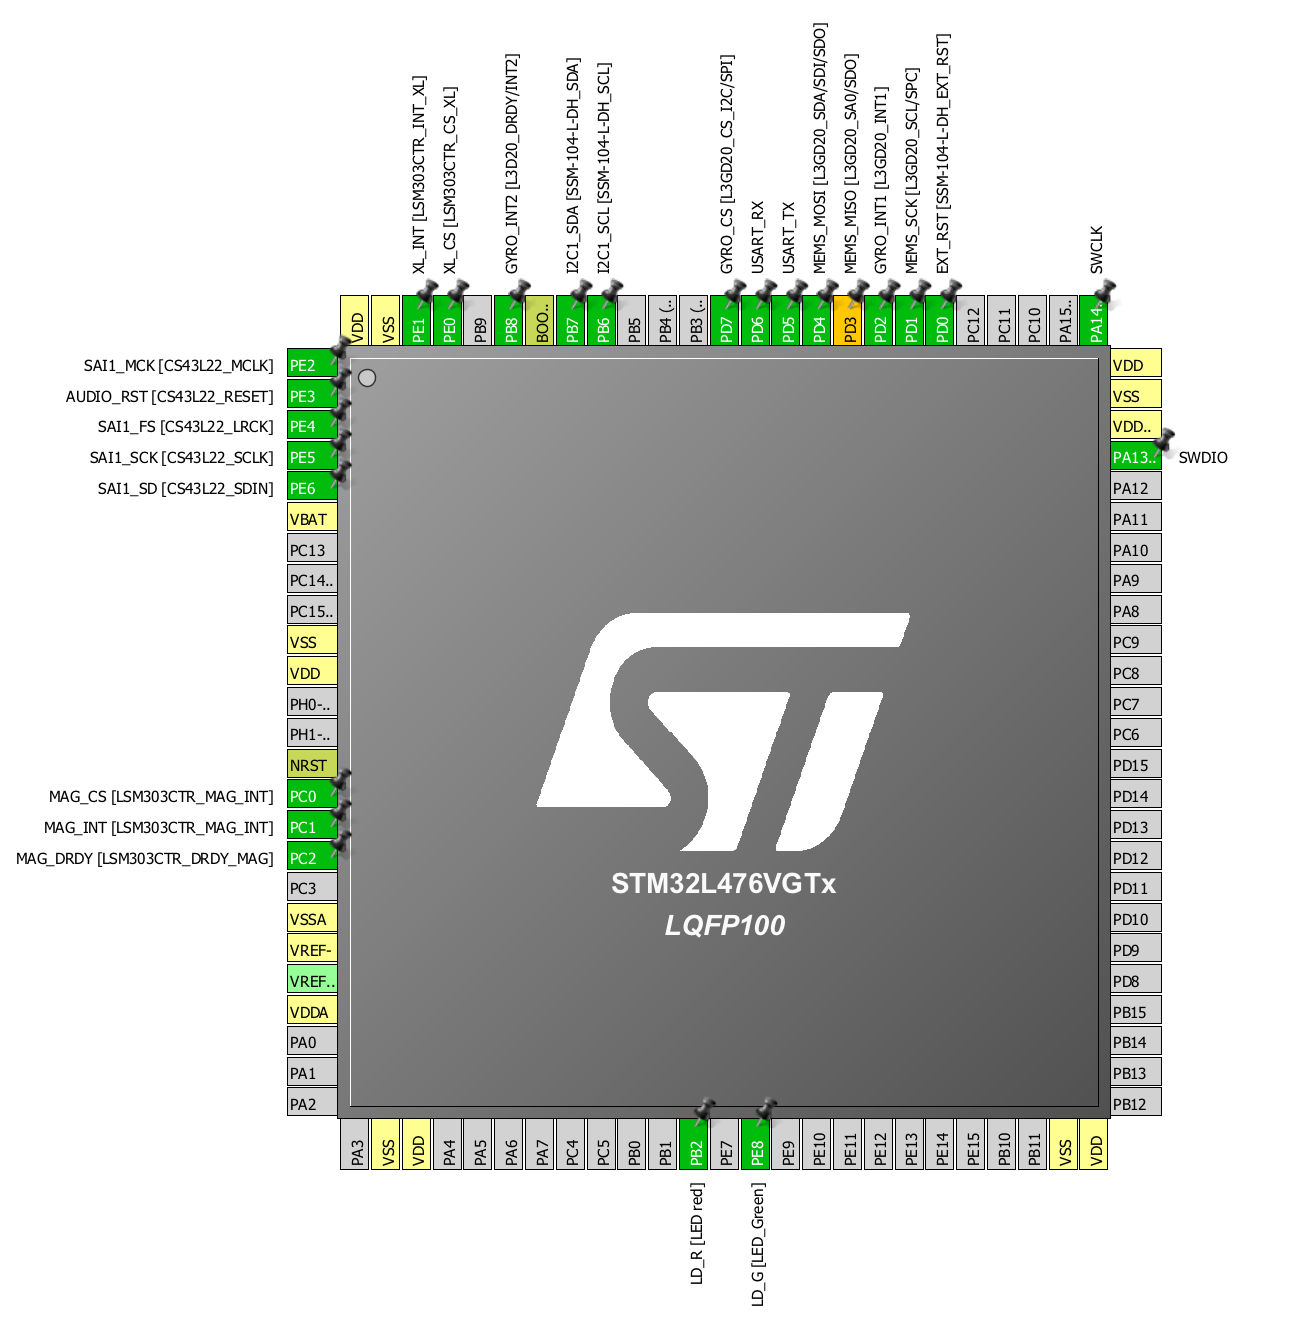
\includegraphics[width=\linewidth]{conf1.png}
	\caption{Konfiguracja pinów}
	\end{figure}


	\begin{figure}[H]
	\centering
	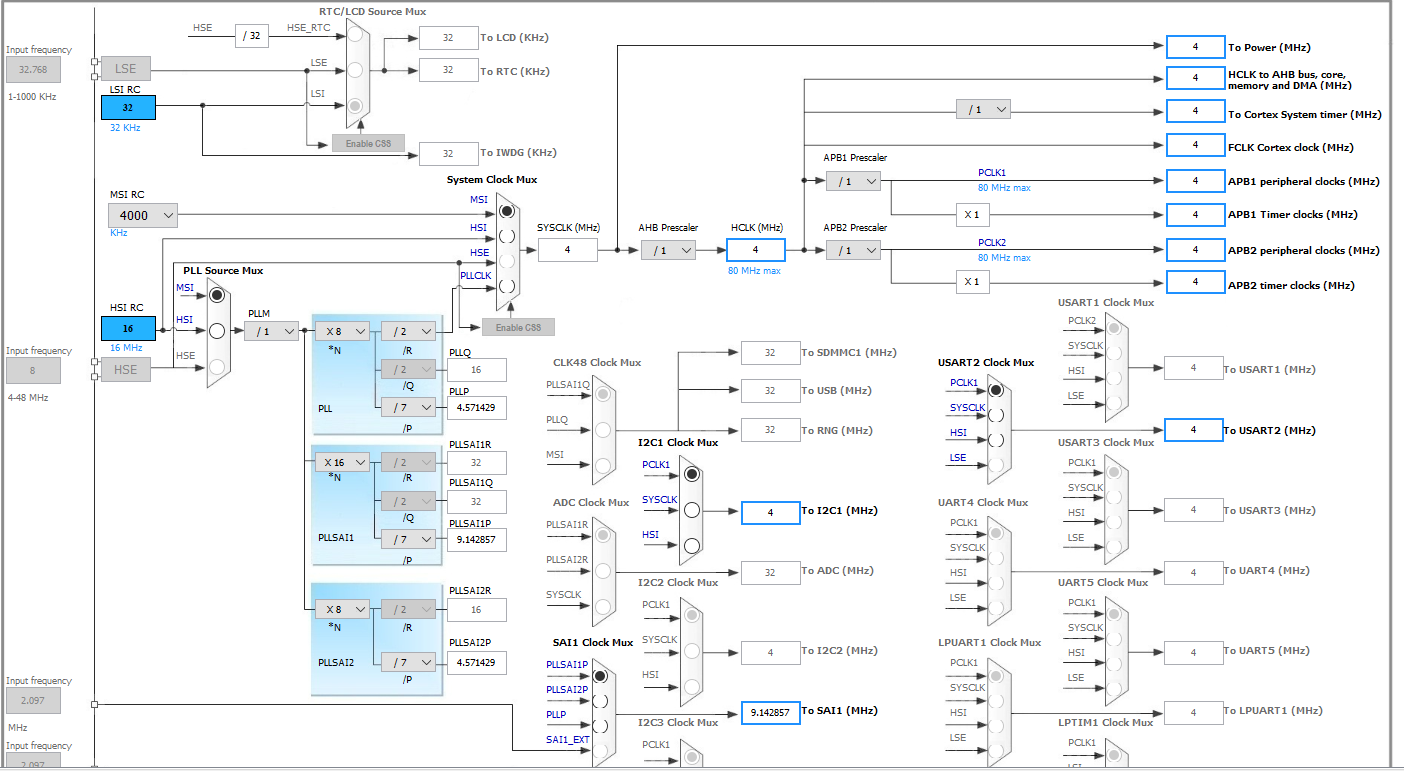
\includegraphics[ width=\textheight,angle=90,keepaspectratio]{conf2.png}
	\caption{Konfiguracja zegarów}
	\end{figure}
\subsection{Konfiguracja pinów}
\begin{figure}[H]
	\centering
	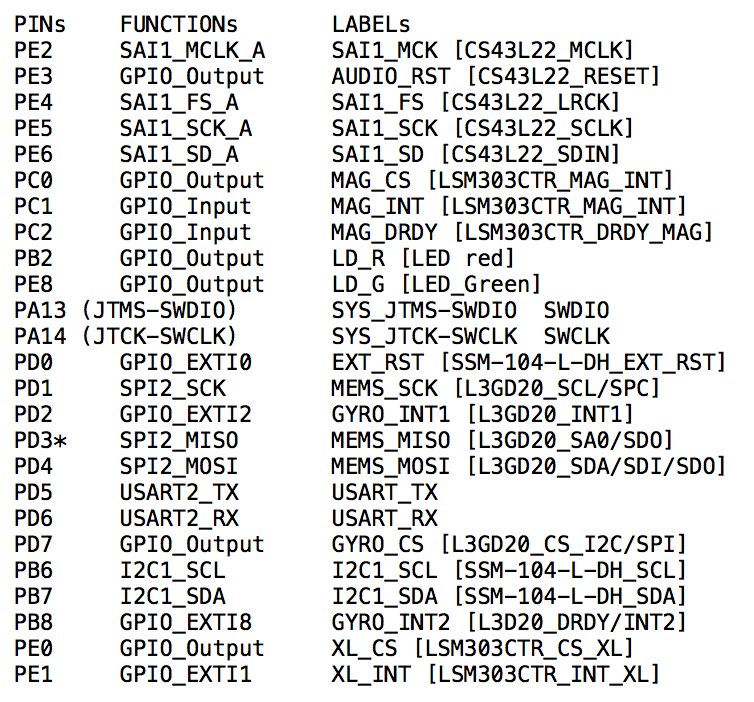
\includegraphics[width=80mm]{conf99.png}
	\caption{Raport z konfiguracji pinów}
	\end{figure}
\subsection{Konfiguracja peryferiów}
W naszym projekcie wykorzystywaliśmy peryferium I2C, I2S oraz SPI. Dokładne dane konfiguracyjne zostały zamieszczone poniżej.
\subsubsection{I2S}
Interfejs szeregowy do przesyłania dźwięku pomiędzy układami scalonymi, domyślna konfiguracja został jedynie zmieniona tylko w rubryce próbkowania dźwięku: z 192kHz na 8kHz. Za pomocą tego interfejsu ukłąd CS43L22 otrzymuje cyfrowy sygnał dźwiękowy który przetwarza na dźwięk.
\subsubsection{I2C}
Magistrala I2C została wykorzystana do konfigurowania oraz kontroli układu CS43L22. Domyślna konfiguracja jest wystarczająca, jedynie prdkość przesyłania danych została zmieniona ze 100kHz na 400kHz. 
\subsubsection{SPI}
Do komunikacji z układem LSM303C musieliśmy użyć SPI w trybie Half-Duplex, ponieważ z dokumentacji wynikało, że układ nie obsługuje komunikacji Full-Duplex. Taka konfiguracja wymusza pracę całej lini w trybie Half-Duplex, a co za tym idzie wszystkich podłączonych do niej układów, w naszym wypadku żyroskopu L3GD20.
\begin{figure}[H]
	\centering
	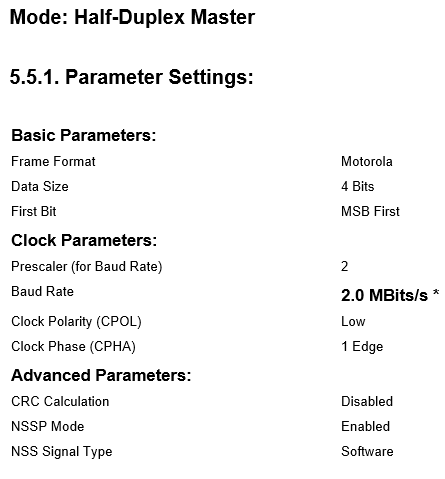
\includegraphics[width=80mm]{c1.png}
	\caption{Konfiguracja SPI}
	\end{figure}




	

\section{Wykorzystane układy zewnętrzne}
\subsection{LSM303C - akcelerometr i magnetometr}
Układ zawiera akcelerometr oraz magnetometr. Jednak do realizacji projektu wykorzystaliśmy sam akcelerometr. Na bieżąco, w trakcie działania programu, przekazuje on odczyty przyśpieszeń z akcelerometru na bazie generowany jest potem dźwięk. Komunikacja odbywa się przez SPI2 w trybie Half-Duplex. Zaimplementowaliśmy filtr górnoprzepustowy oraz odpowiednie zakresy działań miernika. Dla akcelerometru było to 8g (przyśpieszeń ziemskich).




\subsection{L3GD20 - żyroskop}
Układ L3GD20 to urządzenie żyroskopowe, które przekazuje odczyty przyspieszenia kątowego. Wykorzystaliśmy ten MEMS do możliwości odtwarzania dźwięku, gdy miecz obraca się w miejscu. Tutaj też ograniczyliśmy się do prostego odczytywania pomiarów na przerwaniach. Skonfigurowaliśmy go na 2000 DPS. Odczyty z żyroskopu nie są obecnie wykorzystywane.
\subsection{CS43L22 - DAC}
Układ scalony CS43L22 jest układem spełniającym wszystkie potrzeby użytkownika dotyczące przetwarzania sygnału cyfrowego na dźwięk. Układ łączy w sobie DAC, dekoder, wzmacniacz słuchawkowy, wzmacniacz głośnikowy (max 1W na głośnik przy zasilaniu z 5V), DSP pozwalający kontrolować głośność dzwięku, jego tony niskie i wysokie, a także oferuje funkcje limitera i detektora przesterowań, oprócz tego układ potrafi generować piknięcia sygnalizacyjne, a także posiada przejście dźwięku analogowego oraz mixer, zwieńczeniem jest kompensacja zasilania bateryjnego, a więc układ jest idealnym kandydatem do przenośnych aplikacji audio. 

	
	\section{Implementacja obsługi DAC}
Płytka STM32L476G-DISCO wyposażona jest w DAC stereo CS43L22 firmy Cirrus Logic. Do zaprogramowania tego peryferium została wykorzystana biblioteka BSP dostarczona przez firmę ST. Urządzenie to konfigurowane jest przez interfejs I$^2$C, a sygnał audio wysyłany jest przez interfejs SAI. Dane audio są kopiowane z pamięci mikrokontrolera na interfejs SAI z wykorzystaniem układu DMA, pozwala to odciążyć rdzeń mikrokontrolera, a także zapewnić płynność dźwięku. Na tym etapie mikrokontroler generuje przebieg sinusoidalny o konfigurowalnej częstotliwości sygnału, a także o zadanej częstotliwości próbkowania, która nie musi być wysoka z uwagi na to, że wysoka dokładność odwzorowania dźwięku nie jest konieczna, w naszym projekcie częstotliwość próbkowania została ustawiona na 16kHz. Z uwagi na to, że rdzeń generuje dźwięk wolniej niż ten jest odtwarzany konieczne jest zastosowanie osobnego buforu do generowania dźwięku i osobnego do jego odtwarzania, po zakończeniu generowania dźwięku w danym buforze, oraz po zakończeniu odtwarzania próbki wskaźniki na bufory zostana zamienione, dzięki temu procesor będzie mógł generować dźwięk podczas gdy inny dźwięk ( o innej częstotliwości) jest odtwarzany bez przeszkód. Obecnie trwają prace nad stworzeniem formuły która pozwoli syntezować dźwięk miecza świetlnego, gdy prace te zostaną zakończone, formuła zostanie przeniesiona do osobnej funkcji która będzie generować dźwięk na bazie odczytu z akcelerometru do zadanego bufora. Budowa sygnału audio jest bardzo prosta, po ustaleniu częstotliwości próbkowania należy wygenerować tablice amplitud które są typu \textit{uint16\_t} czyli liczby z przedziału od 0 do 65535, biorąc pod uwagę, że jedna sekunda dźwięku składa się z wybranej wcześniej ilości próbek. Cyfrowe filtry DFSDM zostały włączone tylko dlatego, że biblioteka audio BSP ich wymaga, ale nie są one wykorzystywane w tym projekcie.


	\section{Implementacja obsługi akcelerometru i żyroskopu}
	Z powodzeniem udało się zaimplementować obsługę akcelerometru poprzez komunikację SPI. Aby odwzorować ruch miecza w bardziej precyzyjny sposób, postanowiono dodać obsługę poprzez komunikację SPI także żyroskopu. Na płytce STM32L476G-DISCO, żyroskop znajduje się na L3GD20, zaś akcelerometr na LSM303C. Wykorzystano dokumentacje w celu zapoznania się odpowiednia konfiguracja i uruchomieniem tych peryferiów. Dużą pomocą były przykładowe funkcje obsługi tych peryferiów w BSP, opublikowanym przez firmę ST. Obsługę tych urządzeń podzielono na dwie warstwy interfejsu. Pierwsza warstwa to napisane biblioteki accel oraz gyros (.c i .h). Druga warstwa zaś to biblioteki lsm i l3g (.c i .h). Zastosowanie dwóch warstw interfejsu może bardzo pomóc w sytuacji gdy trzeba by było przerobić program do działania na innym sterowniku. W takiej sytuacji nie musimy zmieniać całego programu, tylko jedną warstwę interfejsu. 
Postanowiono ustawić wysokie zakresy działania mierników. Dla żyroskopu była to wartość 2000 DPS (stopnie na sekundę), a dla akcelerometru była to wartość 8G (przyśpieszeń ziemskich). Skalibrowano takie ustawienia by nie dochodziło do saturacji odczytów peryferiów. Inaczej, żeby algorytm proporcjonalnie generował dźwięk ruchu miecza w przestrzeni, nawet przy zamaszystych i szybkich ruchach. 
W projekcie zaimplementowano także biblioteki akcelstruct.h oraz gryostruct.h. Zawierają one struktury do inicjalizacji i konfiguracji tych peryferiów. Ostatnią istotną biblioteką napisaną na potrzebę projektu to komun.h/komun.c. Odpowiedzialna jest ona za skonfigurowanie i przeprowadzenie komunikacji przez kanał SPI2. Biblioteka obsługuje inicjalizację i komunikację z zarówno akcelerometrem jak i żyroskopem. 
W celach testowych, odczyty peryferiów były przesyłane przez komunikację UART na komputer, w różnych odstępach czasu. Wyniki testów zakończyły się powodzeniem. Następnym krokiem będzie dostosowanie wyjściowych zmiennych do potrzeb algorytmu generującego dźwięk w głównej pętli programu. 

\section{Generowanie dźwięku miecza świetlnego}
\subsection{Historia dźwięku z filmów}
Dźwięk miecza świetlnego z filmów \textit{Star Wars} jest połączeniem dźwięku szumu projektora filmowego oraz dźwięku buczenia starego telewizora. Efekt Doppler'a został osiągnięty poprzez odgrywanie dźwięku z głośnika i machanie przed nim mikrofonem zgodnie z ruchami mieczy na filmie.
\subsection{Analiza innych rozwiązań}
Ze znalezionych w sieci rozwiązań większość bazuje na odtwarzaniu sampli z pamięci karty SD. W trybie spoczynkowym jest odtwarzany dźwięk buczenia, podczas ruchu odtwarzany jest prekalkulowany dźwięk potraktowany efektem Doppler'a. Dodatkowym efektem jest dźwięk uderzenia kiedy odczyty z akcelerometru gwałtownie zmieniają się na znak przeciwny. Rozwiązania te nie są zadowalające ponieważ pomiędzy przeładowaniami dźwięku jest odczuwalne opóźnienie oraz dźwięk miecza wydaje się sztuczny z powodu ograniczonej ilości kombinacji (prekalkulowane sample).
\subsection{Generowanie dźwięku i efekt Doppler'a}
 W celu wygenerowania dźwięku miecza świetlnego potrzebna jest częstotliwość generowanego dźwięku. Częstotliwość ta wyliczana jest na podstawie danych odczytanych z akcelerometru. Przyśpieszenie musi być przefiltrowane filtrem górnoprzepustowym w celu odfiltrowania przyśpieszenia ziemskiego. Przyśpieszenie na osiach łączone jest za pomocą średniej kwadratowej, daje nam to bezwzględne przyśpieszenie w przestrzeni. Otrzymana wartość jest następnie całkowana numeryczną całką kwadratową czego wynikiem jest prędkość miecza. Ponieważ miecz jest trzymany przez właściciela i dla niego jest generowany efekt dopplera (jak właściciel miecza porusza się z mieczem to efekt Doppler'a dla innych powstaje naturalnie), to zerowe przyśpieszenie jest równoważne z zerową prędkością miecza względem użytkownika, należy to wziąć pod uwagę i zerować wartość prędkości kiedy przyśpieszenie spadnie poniżej wyznaczonego progu (np. 0,1g). Wyliczona prędkość jest następnie podstawiana do wzoru na efekt dopplera (\ref{eq:dop}) gdzie $v$ to prędkość dźwięku w powietrzu, a, $v_{s}$ to prędkość obiektu względem obserwatora, a wyliczona ze wzoru częstotliwość podawana jest do generatora dźwięku. W obecnym stanie generator generuje sygnał sinusoidalny. Niestety jest on generowany za wolno, aby dało się zauważyć korelację ruchu miecza z częstotliwością dźwięku, prawdopodobnie wynika to z błędnej konfiguracji zegarów, ponieważ mikrokontroler pracował z prędkością jedynie 4MHz, a nie 80MHz tak jak powinien. Nie udało się też odpowiednio oprogramować filtra górnoprzepustowego wbudowanego w akcelerometr. Objawia się to tym, że częstotliwość generowanego sygnału rośnie samoistnie co jakiś czas (ze względu na brak odfiltrowania grawitacji). 
 
 \begin{equation}
 f' = \left(\frac{v}{v-v_{s}}\right)f
 \label{eq:dop}
 \end{equation}
 
 \subsection{Odtwarzanie sampli}
 Kolejnym podejściem do problemu miało być odtwarzania prekalkulowanych sampli lub użycie sampli z gry. W tym celu wykorzystano program \textit{Cubase} w celu obrobienia i przycięcia sampli, a nastepnie za pomocą pakietu \textit{Matlab} przetworzono pliki WAV na liczby \textit{uint16\_t}. Tak przygotowane sample wgrano do mikrokontrolera jako \textit{Look Up Table}. Wskaźnik odtwarzani przełącza się pomiędzy tablicami w zależności od przyśpieszenia w przestrzeni odczytanego z akcelerometru. Sample jednak nie są odtwarzane z odpowiednią jakością, może to byc przyczyną próbkowania z częstotliwością jedynie 8kHz, jednak ten sam sampel odtwarza się na komputerze z zadowalającą jakością.



\section{Konstrukcja miecza świetlnego}	


Fizycznie miecz świetlny jest konstrukcją wykorzystującą specjalnie zamówioną rurę plexi. Rura ma długość 1 m  i zewnętrzną średnicą ok. 34 mm. Grubość rury dobrano na 3 mm. Włożona została do rękojeści i wpasowana w specjalnie wycięte drewniane pierścienie stabilizacyjneo średnicy wewnętrznej 40 mm oraz zewnętrznej 60 mm. Aby można było wpasować rurę plexi do pierścieni stabilizacyjnych, należało wpierw sfazować jej jeden koniec.\\	
\begin{figure}[H]
	\centering
	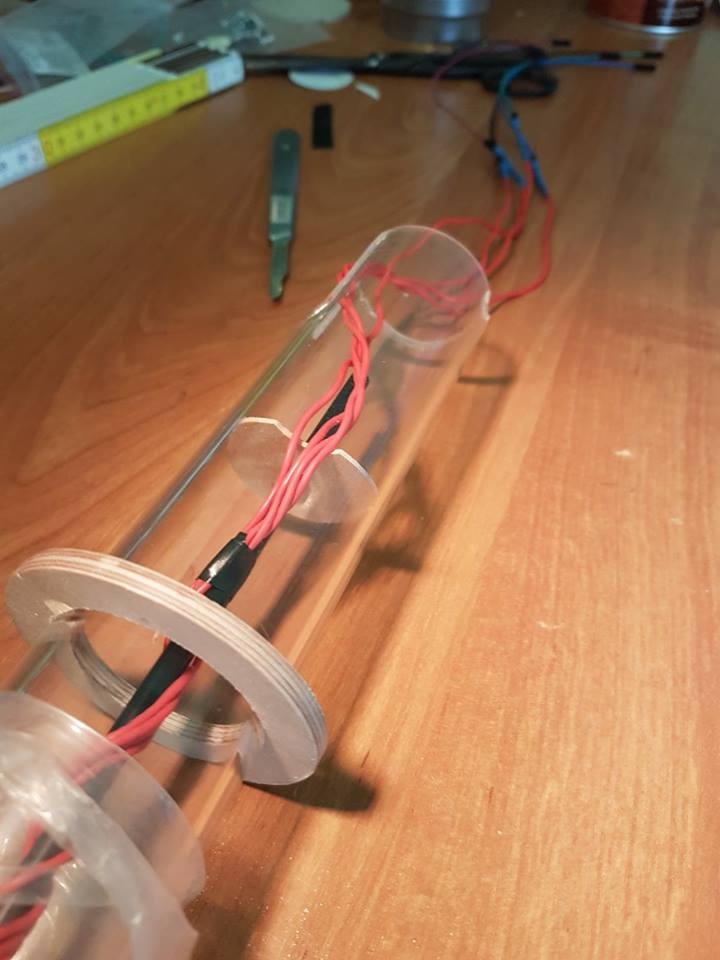
\includegraphics[width=60mm]{11.jpg}
	\end{figure}
	\begin{figure}[H]
	\centering
	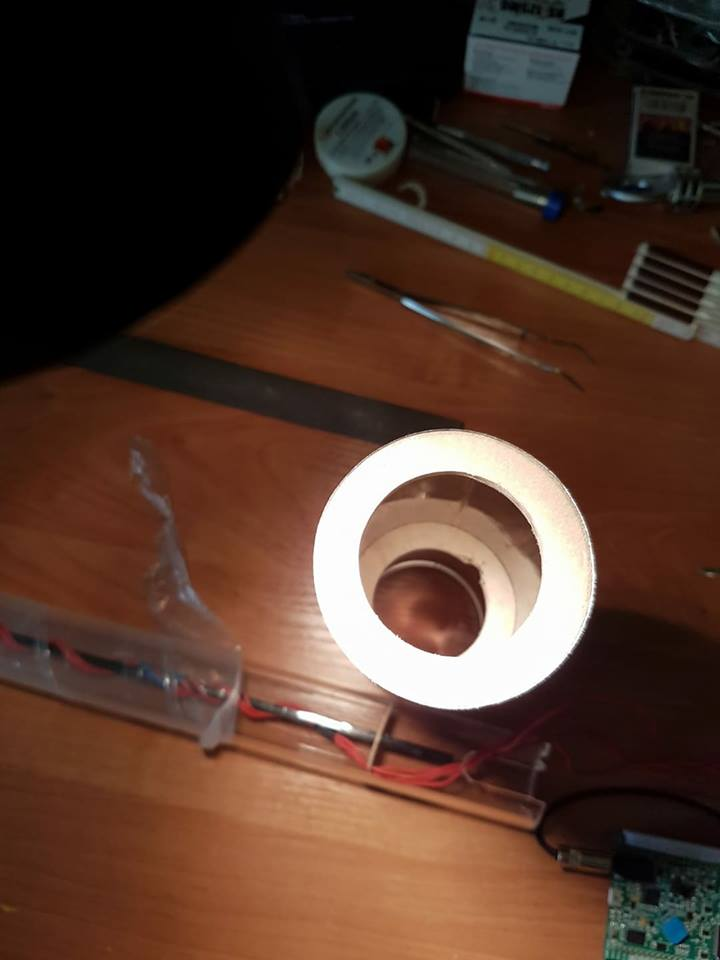
\includegraphics[width=60mm]{12.jpg}
	\end{figure}
Rękojeść została zrealizowana z metalowej rury o średnicy 60 mm oraz długości 250 mm. W środku znajduje się mikrokontroler STM32L476G-DISCO odpowiedzialny za generowanie dźwięku na bazie odczytów z akcelerometru oraz żyroskopu. Sterownik został zamocowany na gąbkach zwiększających tarcie. Średnica rury została dobrana do szerokości mikrkontrolera. Dzięki temu mikrokontroler stabilnie utrzymuje swoją pozycję w rękojeści bez konieczności klejenia bądź innego rodzaju mocowania. 
\begin{figure}[H]
	\centering
	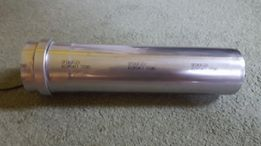
\includegraphics[width=60mm]{4.jpg}
	\end{figure}
	\begin{figure}[H]
	\centering
	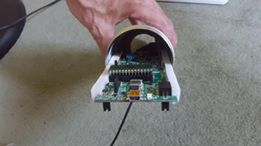
\includegraphics[width=60mm]{6.jpg}
	\end{figure}
Podłączony jest do niego też głośnik Tracer Stream BT, który będzie wydawał generowane przez mikrokontroler dźwięki.\\
W dolny otwór rury rękojeści została wkręcona listwa. W nią wkręcono trzy śruby mające na dystansach połączyć rękojeść z dolną częścią miecza. Jest nią puszka, która w środku ma dwa istotne elementy. Wcześniej wspomniany głośnik Tracer Stream BT oraz płytka STM32 NUCLEO-F103RB.\\ 
	\begin{figure}[H]
	\centering
	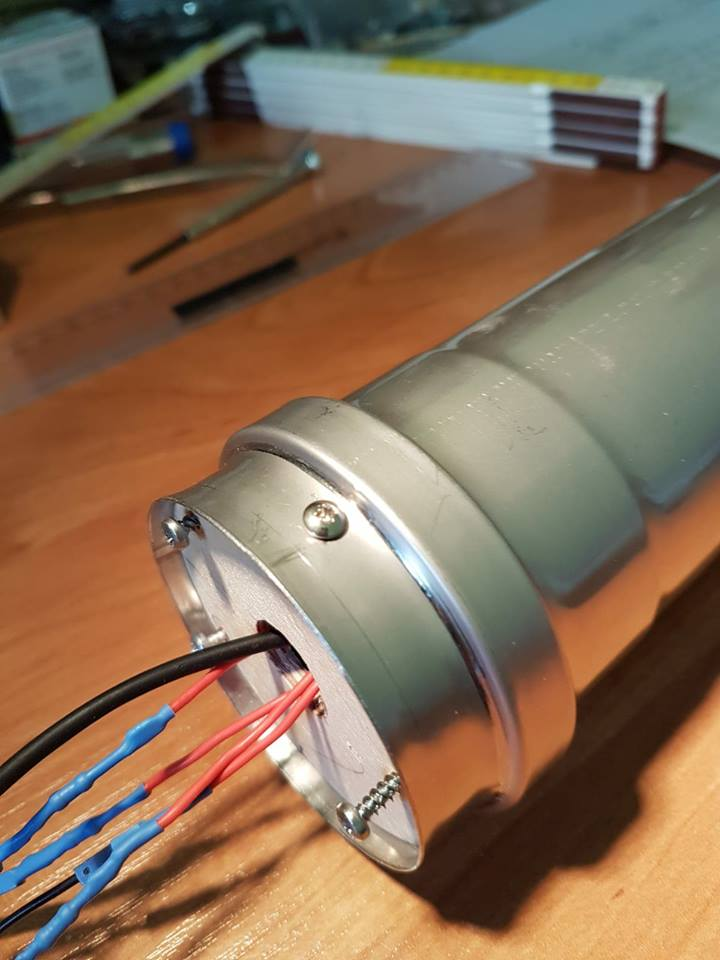
\includegraphics[width=60mm]{13.jpg}
	\end{figure}
		\begin{figure}[H]
	\centering
	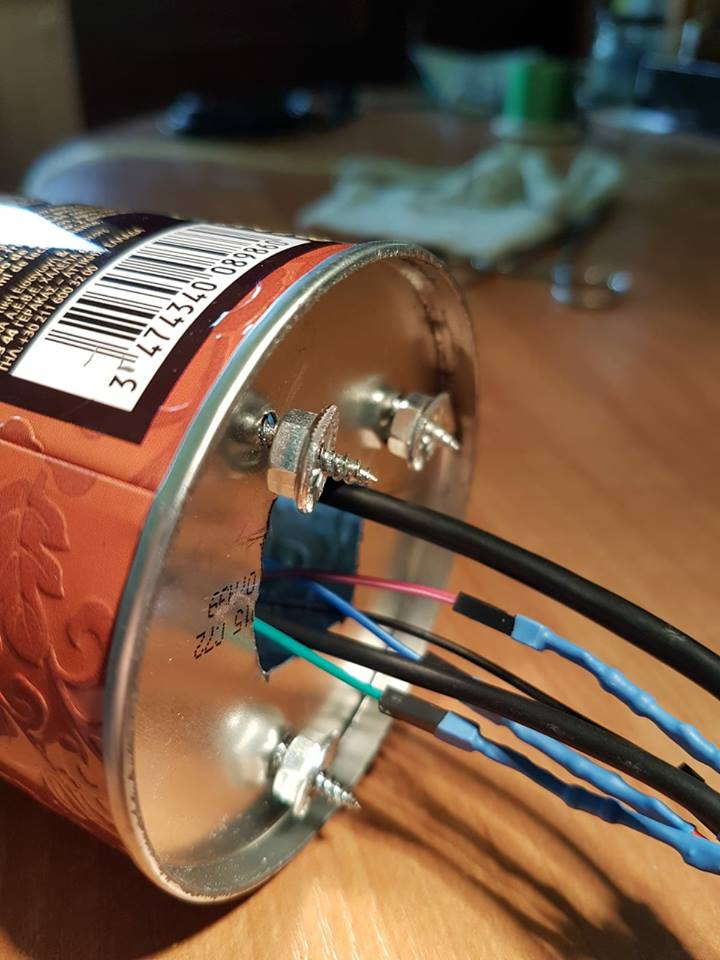
\includegraphics[width=60mm]{19.jpg}
	\end{figure}
		\begin{figure}[H]
	\centering
	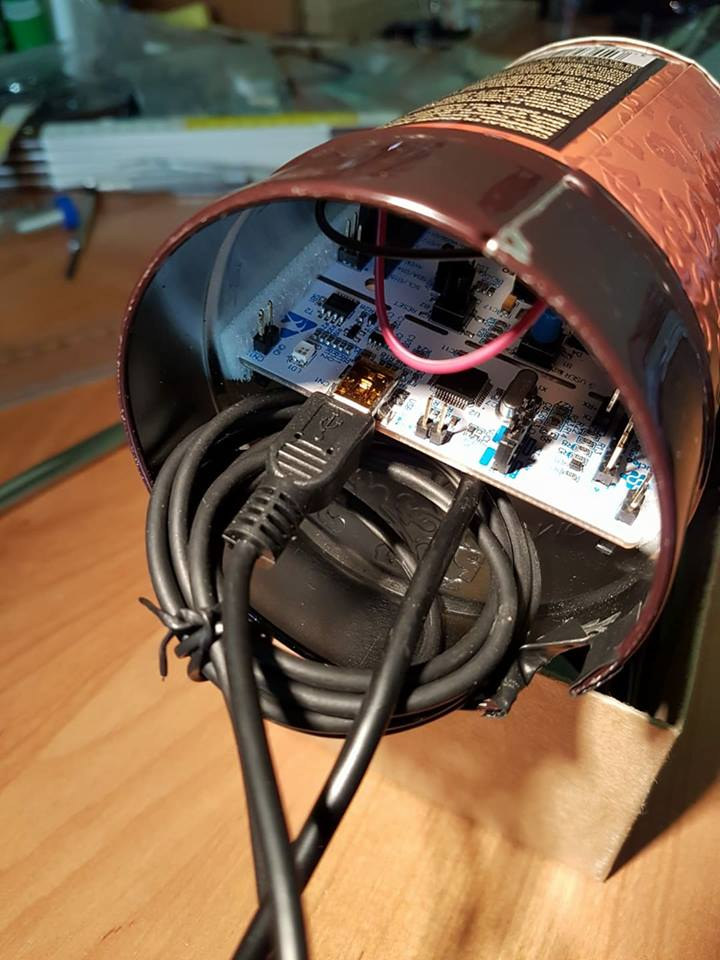
\includegraphics[width=40mm]{21.jpg}
	\end{figure}
Drugą płytkę wykorzystana w celu interfejsu UART, dzięki któremu można sterować kolorem diod LED RGB, stanowiących oświetlenie miecza. Do zasilenia tego układu korzystamy z zasilania USB, zaś układem 5 diod RGB sterujemy sygnałem PWM. Do konfiguracji płytki NUCLEO nie wykorzystana z programu CUBE. Całą konfiguracja została napisana ręcznie na niskim poziomie. 
\lstinputlisting[firstline = 3,caption=Konfiguracja,language=C++]
{k.cpp}
\lstinputlisting[firstline = 3,caption=Interfejs UART,language=C++]
{u.cpp}
Głośnik Tracer będzie przymocowany na zewnątrz puszki. Dzięki temu wygenerowane odgłosy nie będą zagłuszane w żaden sposób. Mocowanie odbyło się za pomocą skręconych ze sobą trzech listw miękkich zatrzaskujących się na nóżce głośnika. \\
	\begin{figure}[H]
	\centering
	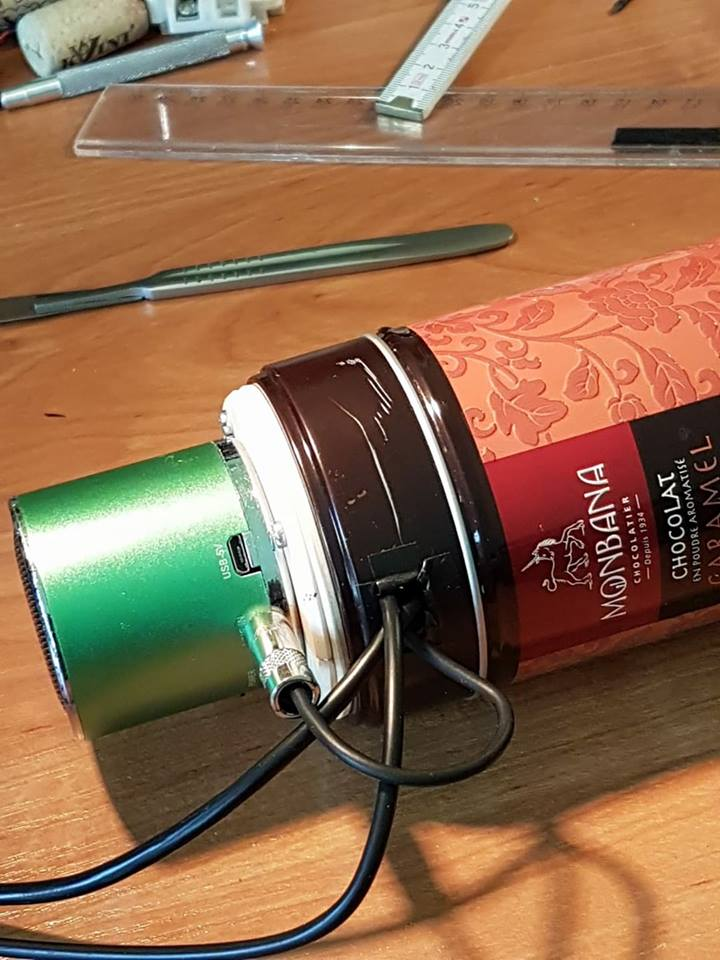
\includegraphics[width=40mm]{9.jpg}
	\end{figure}
Do komunikacji i zasilenia płytek wykorzystany zostanie układ kabli miniUSB z przedłużaczami USB o całkowitej długości ok. 3 m. Dzięki takiemu rozwiązaniu, użytkownik nie będzie ograniczany przy poruszaniu mieczem. \\
Oświetlenie miecza zostało zrealizowane na bazie pięciu prostych diod LED RGB o wspólnej anodzie oraz zamglonym szkiełku. Każdy moduł RGB, we wszystkich diodach na raz, sterujemy sygnałem PWM. Zlutowany układ został przymocowany do cienkiej węglowej rurki. Po podłączeniu układu do odpowiedniej płytki, diody zostały wprowadzone na węglowej rurce do wnętrza rury plexi. \\
	\begin{figure}[H]
	\centering
	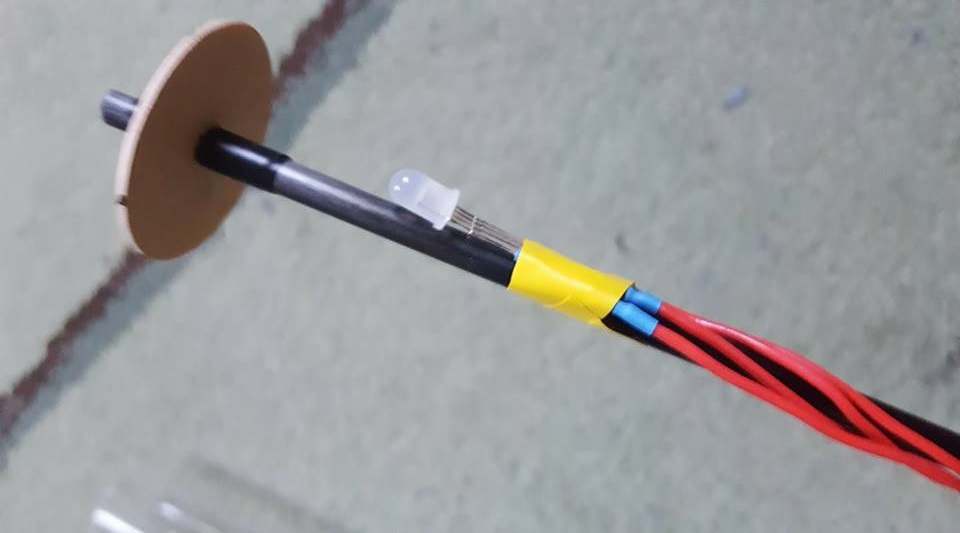
\includegraphics[width=100mm]{3.jpg}
	\end{figure}
		\begin{figure}[H]
	\centering
	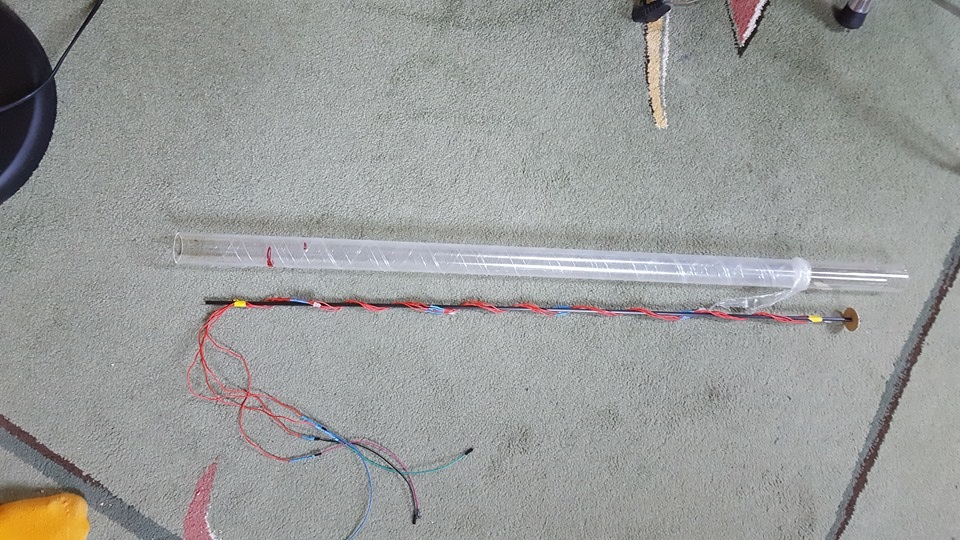
\includegraphics[width=100mm]{2.jpg}
	\end{figure}
Cała konstrukcja jest solidna i wytrzymała na wstrząsy. W przypadku posiadania drugiego miecza, możliwe jest umyślne dokonywanie kolizji między nimi. Jednocześnie rozmiary miecza i jego waga nie obciążają użytkownika trzymającego miecz. \\

Wadą konstrukcji jest szerokość rękojeści, która została wymuszona przez szerokość płytki STM32L476G-DISCO. Założenia projektowe od początku zakładały wykorzystanie akcelerometru i żyroskopu znajdującego się na tej płytce. Dlatego należało zlokalizować ją jak najbliżej miejsca uchwytu dla dłoni. Zaletą jednak sytuacji jest to, że płytka STM32L476G-DISCO jest wyjątkowo wąska w stosunku do innych modeli, np. STM32F411VET6. Słabym punktem w konstrukcji mechanicznej może się okazać też połączenie między rękojeścią a puszką. Istnieje szansa, że przy odpowiednim nacisku bocznym, doszłoby do wyłamania śrub z listwy bądź z puszki. Jednak przy testowaniu takiego scenariusza nie doszło do żadnego wypadku. Poniżej zamieszczone zostało zdjęcie konstrukcji mechanicznej.
	\begin{figure}[H]
		\centering
	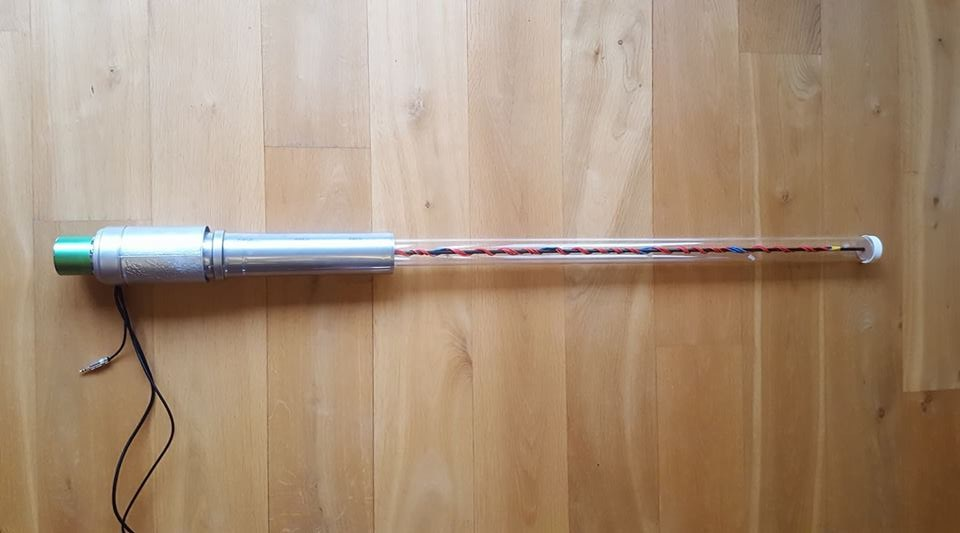
\includegraphics[width=120mm]{22.jpg}
	\end{figure}
\section{Wnioski}
Pomimo tego, że nie udało się w pełni zrealizować założeń, projekt pozwolił zapoznać się z problemami towarzyszącymi przy generowaniu i odtwarzaniu dźwięków na systemach wbudowanych. O ile mikrokontroler jest w stanie generować dźwięk to ważnym jest, żeby taktowanie rdzenia było jak najwyższe ponieważ są to obliczenia czysto matematyczne i ciężko zrealizować takie operacje sprzętowo na zwykłych mikrokontrolerach, dodatkowym atutem jest sprzętowe wsparcie dla liczb zmiennoprzecinkowych. Kiedy pożądane jest odtwarzanie sampli, należy wykorzystać zewnętrzną szybką pamięć do ich przechowywania, żeby nie marnować pamięci RAM, warto rozważyć mikrokontroler z interfejsem SDIO który pozwoli podłączyć kartę pamięci SD szybkim 4 bitowym łączem szeregowym, a także pozwoli na bezbolesną zmianę sampli za pomocą komputera. Ładowanie sampli do pamięci RAM za pomocą układu DMA, a następnie do interfejsu I2S z pamięci RAM także za pomocą DMA pozwoli odciążyć rdzeń, a także zapewnić płynność odtwarzanemu dźwięku. Problemowa okazała się także komunikacja przez SPI w trybie Half-Duplex, lepszym rozwiązaniem jest użycie scalonych układów IMU i komunikacja z nimi za pomocą SPI Full-Duplex lub I2C, taki interfejs da się zaprogramować w pare godzin.
\section{Źródła}
\begin{itemize}
\item https://www.artekit.eu/diy-lightsaber-audio-board/
\item https://www.pbs.org/video/shanks-fx-lightsaber-audio/
\item https://github.com/sidlebj/ECE387Final/wiki
\item http://www.instructables.com/id/Arduino-Based-Lightsaber-With-Light-and-Sound-Effe/
\item http://www.instructables.com/id/Make-Lightsaber-With-Sound-Effectby-Arduino/
\item http://www.carlosvadillo.com/?page\_id=21
\item https://github.com/neskweek/LightSaberOS
\item https://www.silabs.com/community/blog.entry.html/2016/12/14/build\_your\_own\_light-kc4a
\item https://stackoverflow.com/questions/12089662/mixing-16-bit-linear-pcm-streams-and-avoiding-clipping-overflow
\item https://dsp.stackexchange.com/questions/3581/algorithms-to-mix-audio-signals-without-clipping
\item http://atastypixel.com/blog/how-to-mix-audio-samples-properly-on-ios/
\item https://www.thermaxxjackets.com/doppler-effect-frequency-change/
\item https://formulas.tutorvista.com/physics/doppler-shift-formula.html
\item http://hyperphysics.phy-astr.gsu.edu/hbase/Sound/dopp.html
\end{itemize}



\newpage
\addcontentsline{toc}{section}{Bibilografia}
\bibliography{bibliografia}
\bibliographystyle{plain}


\end{document}







































